% ============================================================
% main.tex — VBM Analysis of Cortical Structure across the Adult Lifespan
% ============================================================
\documentclass[12pt, a4paper]{article}

% ---- Encoding & Fonts ----
\usepackage[utf8]{inputenc}
\usepackage[T1]{fontenc}
\usepackage{mathptmx}            % Times Roman for body text

% ---- Page Layout ----
\usepackage[margin=1in]{geometry}
\usepackage{setspace}
\doublespacing

% ---- Language & Typography ----
\usepackage[english]{babel}
\usepackage{microtype}

% ---- Mathematics ----
\usepackage{amsmath, amssymb}

% ---- Tables ----
\usepackage{booktabs}            % Professional-quality horizontal rules
\usepackage{tabularx}            % Full-width tables with X columns
\usepackage{multirow}            % Cells spanning multiple rows
\usepackage{makecell}            % Line breaks inside cells
\usepackage{longtable}           % Multi-page tables
\usepackage{array}               % Extended column specifications
\usepackage{siunitx}             % Decimal-aligned columns

% ---- Figures & Graphics ----
\usepackage{graphicx}
\graphicspath{{../results/figures/}}
\usepackage{subcaption}          % Sub-figures (a), (b), (c)
\usepackage{float}               % Exact float placement [H]

% ---- Colors ----
\usepackage[dvipsnames]{xcolor}

% ---- Captions ----
\usepackage[font=small, labelfont=bf, labelsep=period]{caption}

% ---- Lists ----
\usepackage{enumitem}

% ---- Cross-references & Hyperlinks ----
\usepackage[colorlinks=true,
            linkcolor=MidnightBlue,
            citecolor=MidnightBlue,
            urlcolor=MidnightBlue]{hyperref}

% ---- Bibliography (inline thebibliography, no .bib needed) ----

% ---- Line Numbers (for review) ----
\usepackage{lineno}

% ---- Section Header Formatting ----
\usepackage{titlesec}
\titleformat{\section}{\normalfont\Large\bfseries}{\thesection.}{0.5em}{}
\titleformat{\subsection}{\normalfont\large\bfseries}{\thesubsection.}{0.5em}{}
\titleformat{\subsubsection}{\normalfont\normalsize\bfseries}{\thesubsubsection.}{0.5em}{}

% ---- Compact Spacing for Display Equations ----
\AtBeginDocument{%
  \abovedisplayskip=8pt plus 2pt minus 4pt
  \belowdisplayskip=8pt plus 2pt minus 4pt
}

% ============================================================
% Document Metadata
% ============================================================
\title{\textbf{Cortical Morphometry across Behavior and Age:\\
A Dual-Cohort Study of Sleep, Cognition, Personality,\\
and Lifespan Structural Change}}

\author{%
  Author Name \\
  \textit{Department of Cognitive Neuroscience} \\
  \textit{University Name} \\
  \texttt{author@university.edu}
}

\date{}

% ============================================================
\begin{document}

\maketitle

% ---- Abstract ----
% ============================================================
% abstract.tex
% ============================================================

\begin{abstract}
\noindent
Understanding how behavioral traits relate to cortical morphometry, and how those relationships shift with age, is a central question in human neuroscience.
We present a dual-cohort analysis that examines sleep quality, fluid intelligence, and neuroticism as predictors of cortical thickness and surface area, alongside a characterization of age-related cortical decline.
Using the Human Connectome Project Young Adult dataset (\textit{N}\,=\,1{,}104; ages 22--37; Desikan-Killiany atlas, 68 regions of interest) and the Aging Brain and Behaviour Cohort (\textit{N}\,=\,1{,}150; ages 36--89; Glasser HCP-MMP1 atlas, 360 regions of interest), we conducted region-wise Welch \textit{t}-tests, Pearson correlations, and one-way ANOVAs, applying Benjamini-Hochberg false discovery rate correction throughout.
Three principal findings emerged: (1)~fluid intelligence correlated positively with surface area across all 68 regions in young adults; (2)~cortical thickness and volume declined near-universally with age, with the strongest effects in primary motor cortex (\textit{r}\,=\,$-$0.69); and (3)~neuroticism was associated with widespread cortical thinning in the aging cohort (327 of 360 regions) but not in young adults, suggesting that cumulative stress exposure may be required for structural differences to manifest.
These results underscore the importance of cohort-specific designs when investigating brain-behavior associations and provide converging evidence that the aging cortex is differentially vulnerable to personality-linked physiological processes.
\end{abstract}

\vspace{0.5cm}
\noindent\textbf{Keywords:} cortical thickness, surface area, voxel-based morphometry, aging, sleep quality, fluid intelligence, neuroticism, Human Connectome Project
\newpage


% ---- Introduction ----
% ============================================================
% introduction.tex
% ============================================================

\section{Introduction}
\label{sec:introduction}

The human cerebral cortex undergoes measurable structural change throughout the adult lifespan. Cortical thickness decreases in a regionally heterogeneous pattern that accelerates after the fifth decade~\cite{fjell2010structural, salat2004thinning}, cortical surface area follows a largely independent developmental trajectory~\cite{storsve2014differential}, and cortical volume, which reflects the product of the two, declines across nearly every parcellated region by late adulthood~\cite{raz2005regional}. These morphometric indices are not merely markers of biological aging; they covary with cognitive ability~\cite{deary2010neuroscience}, affective temperament~\cite{riccelli2017surface}, and health-relevant behaviors such as habitual sleep quality~\cite{sexton2014poor}. A growing body of work therefore treats cortical morphometry as a common endpoint through which disparate behavioral and demographic factors can be compared on a shared anatomical scale.

Despite this convergence of interest, most studies examine a single behavioral predictor in a single sample and report effects in one cortical metric. Sleep quality has been linked to regional thinning in temporal and frontal areas in community-dwelling older adults~\cite{sexton2014poor, branger2016relationships}, but few studies have tested the same association in a young-adult cohort with restricted age variance, where the contribution of age-related confounds is minimized. Fluid intelligence correlates positively with total brain volume and, to a lesser extent, with regional gray matter density~\cite{pietschnig2015meta, colom2009human}; yet the specific relationship between intelligence and cortical \textit{surface area}, as opposed to thickness, remains underexplored in large samples despite theoretical grounds for expecting such an association~\cite{jung2007pfit}. Neuroticism, the personality dimension most consistently linked to negative affect and stress reactivity~\cite{costa1992neo}, has been associated with both thicker and thinner cortices depending on participant age, brain region, and imaging modality~\cite{bjornebekk2013neuronal, jackson2011cortical}, leaving open the question of whether these effects are present in young adulthood or instead emerge only with prolonged exposure to stress-related physiological processes~\cite{lupien2009effects}. In short, there is no single study that examines sleep, cognition, and personality within the same analytic framework while simultaneously characterizing age-related cortical decline across a complementary lifespan sample.

The present work addresses this gap through a dual-cohort design. We use the Human Connectome Project Young Adult (HCP-YA) dataset~\cite{vanessen2013wuminn}, which provides high-resolution structural MRI and extensive behavioral phenotyping for 1{,}104 adults aged 22 to 37, to investigate three research questions: whether subjective sleep quality (Pittsburgh Sleep Quality Index; PSQI~\cite{buysse1989pittsburgh}) predicts regional cortical thickness, whether fluid intelligence (Penn Progressive Matrices) predicts cortical surface area, and whether dispositional neuroticism (NEO Five-Factor Inventory~\cite{costa1992neo}) predicts either metric. For the HCP cohort, structural data are parcellated using the Desikan-Killiany atlas~\cite{desikan2006automated}, yielding 34 regions per hemisphere (68 total). We then turn to the Aging Brain and Behaviour Cohort (AABC Release~2)~\cite{bookheimer2019aging}, which includes 1{,}150 adults spanning ages 36 to 89, parcellated with the finer-grained Glasser HCP-MMP1 atlas~\cite{glasser2016multimodal} (180 regions per hemisphere). In this older cohort, we characterize the regional pattern of age-related thickness and volume decline and test whether sleep quality and neuroticism continue to predict cortical structure after the dominant contribution of age has been accounted for.

Across both cohorts, we apply a uniform analytic strategy. Group comparisons use Welch's \textit{t}-test, continuous associations are assessed with Pearson's correlation, and all \textit{p}-values are adjusted for multiplicity using the Benjamini-Hochberg false discovery rate procedure at \textit{q}\,<\,.05~\cite{benjamini1995controlling}. Effect sizes are reported as Cohen's \textit{d} for group contrasts and as Pearson's \textit{r} for correlational analyses, with 95\% confidence intervals throughout. This consistent framework enables direct comparison of effect magnitudes across research questions.

Three principal findings emerge from this work. First, fluid intelligence showed a positive association with cortical surface area in every region tested, with the largest effects concentrated in the inferior and middle temporal cortex. Second, cortical thickness and volume declined with age across nearly all 360 Glasser regions, with primary motor cortex exhibiting the single strongest effect (\textit{r}\,=\,$-$0.69 for thickness). Third, neuroticism was unrelated to cortical thickness in young adults (0 of 68 regions survived FDR correction) but was associated with widespread thinning in the aging cohort (327 of 360 regions, Cohen's \textit{d} up to $-$0.39), suggesting that the structural correlates of this personality trait accumulate with age. Conversely, sleep quality showed a modest three-region effect in young adults and no surviving associations in the aging sample, where age itself accounted for the overwhelming majority of variance in cortical structure.

These findings carry two implications for the broader field. Methodologically, they demonstrate that the same behavioral variable can yield opposing conclusions depending on the age composition of the sample and the cortical metric under examination, reinforcing the need for multi-cohort, multi-metric designs. Substantively, the divergent age profiles for neuroticism and sleep quality suggest that the biological pathways linking personality to cortical structure may involve chronic, cumulative processes, such as hypothalamic-pituitary-adrenal axis dysregulation and elevated allostatic load~\cite{mcewen2006protective}, that require decades to leave a detectable morphometric signature.


% ---- Methods ----
% ============================================================
% methods.tex
% ============================================================

\section{Methods}
\label{sec:methods}

\subsection{Participants and Datasets}
\label{sec:methods-data}

Two publicly available datasets were used, chosen to span complementary segments of the adult lifespan and to provide well-validated behavioral phenotyping alongside high-resolution structural MRI.

\subsubsection{Human Connectome Project -- Young Adult (HCP-YA)}

The HCP-YA dataset~\cite{vanessen2013wuminn} comprises healthy adults aged 22 to 37 who were recruited as part of the WU-Minn consortium.
After excluding participants with missing values on any analysis variable (sleep quality, fluid intelligence, neuroticism, or FreeSurfer-derived structural metrics), the final analytic sample consisted of \textit{N}\,=\,1{,}104 individuals.
Participants completed the Pittsburgh Sleep Quality Index (PSQI;~\cite{buysse1989pittsburgh}), providing a global sleep-quality score with higher values indicating poorer sleep; the Penn Progressive Matrices (PMAT24\_A\_CR), a measure of fluid reasoning; and the NEO Five-Factor Inventory neuroticism subscale (NEOFAC\_N;~\cite{costa1992neo}).
Each participant's T1-weighted MRI was processed through the FreeSurfer pipeline~\cite{fischl2012freesurfer}, yielding estimates of regional cortical thickness and cortical surface area for 34 regions per hemisphere (68 total) based on the Desikan-Killiany (DK) atlas~\cite{desikan2006automated}.
Only baseline-visit scans were retained when multiple visits were available.
Age was recorded in bins (e.g., 22--25, 26--30, 31--35); we used the midpoint of each bin for descriptive purposes.

\subsubsection{Aging Brain and Behaviour Cohort (AABC Release 2)}

The AABC study~\cite{bookheimer2019aging} recruited a community-dwelling sample spanning ages 36 to 89, with data acquired across multiple sites as part of the Lifespan Human Connectome Project in Aging.
Structural MRI data were processed using FreeSurfer, and cortical parcellation followed the Glasser HCP-MMP1 atlas~\cite{glasser2016multimodal}, which subdivides each hemisphere into 180 cytoarchitectonically defined regions (360 total).
Behavioral data were obtained from the extended non-imaging battery, which includes the PSQI global sleep-quality score and the NEO neuroticism subscale.
After merging demographic, behavioral, and structural data and retaining only baseline visits, the final sample comprised \textit{N}\,=\,1{,}150 participants.
Age was recorded as a continuous variable, and for ANOVA analyses, participants were binned into decades (30s, 40s, 50s, 60s, 70s, 80+).

\subsection{Cortical Parcellation Atlases}
\label{sec:methods-atlases}

The two datasets employ different parcellation schemes, which differ in spatial resolution and in the principles underlying region definition.
The Desikan-Killiany atlas~\cite{desikan2006automated} defines 34 gyral-based regions per hemisphere on the basis of macroanatomical landmarks; it is widely used in clinical and population-level studies owing to its high test-retest reliability across scanners.
The Glasser HCP-MMP1 atlas~\cite{glasser2016multimodal} defines 180 regions per hemisphere using multimodal boundaries derived from cortical architecture, function, connectivity, and topography; it offers substantially finer granularity but requires high-quality data for accurate parcellation.
Because the two atlases partition the cortex at different spatial scales, region-level results cannot be compared directly.
To facilitate cross-dataset interpretation, we constructed a lobe-level correspondence table that maps each DK region and each Glasser region to one of five canonical lobes (Frontal, Parietal, Temporal, Occipital, Insular).
For DK regions in the cingulate cortex, anterior cingulate regions were assigned to the Frontal lobe and posterior/isthmus cingulate regions were assigned to the Parietal lobe, consistent with cytoarchitectonic conventions used in the Glasser atlas.
The resulting lobe-level mapping is visualized in Figure~\ref{fig:atlas-lobe}, which renders both atlases on the fsaverage inflated surface with shared lobe coloring.

\begin{figure}[htbp]
  \centering
  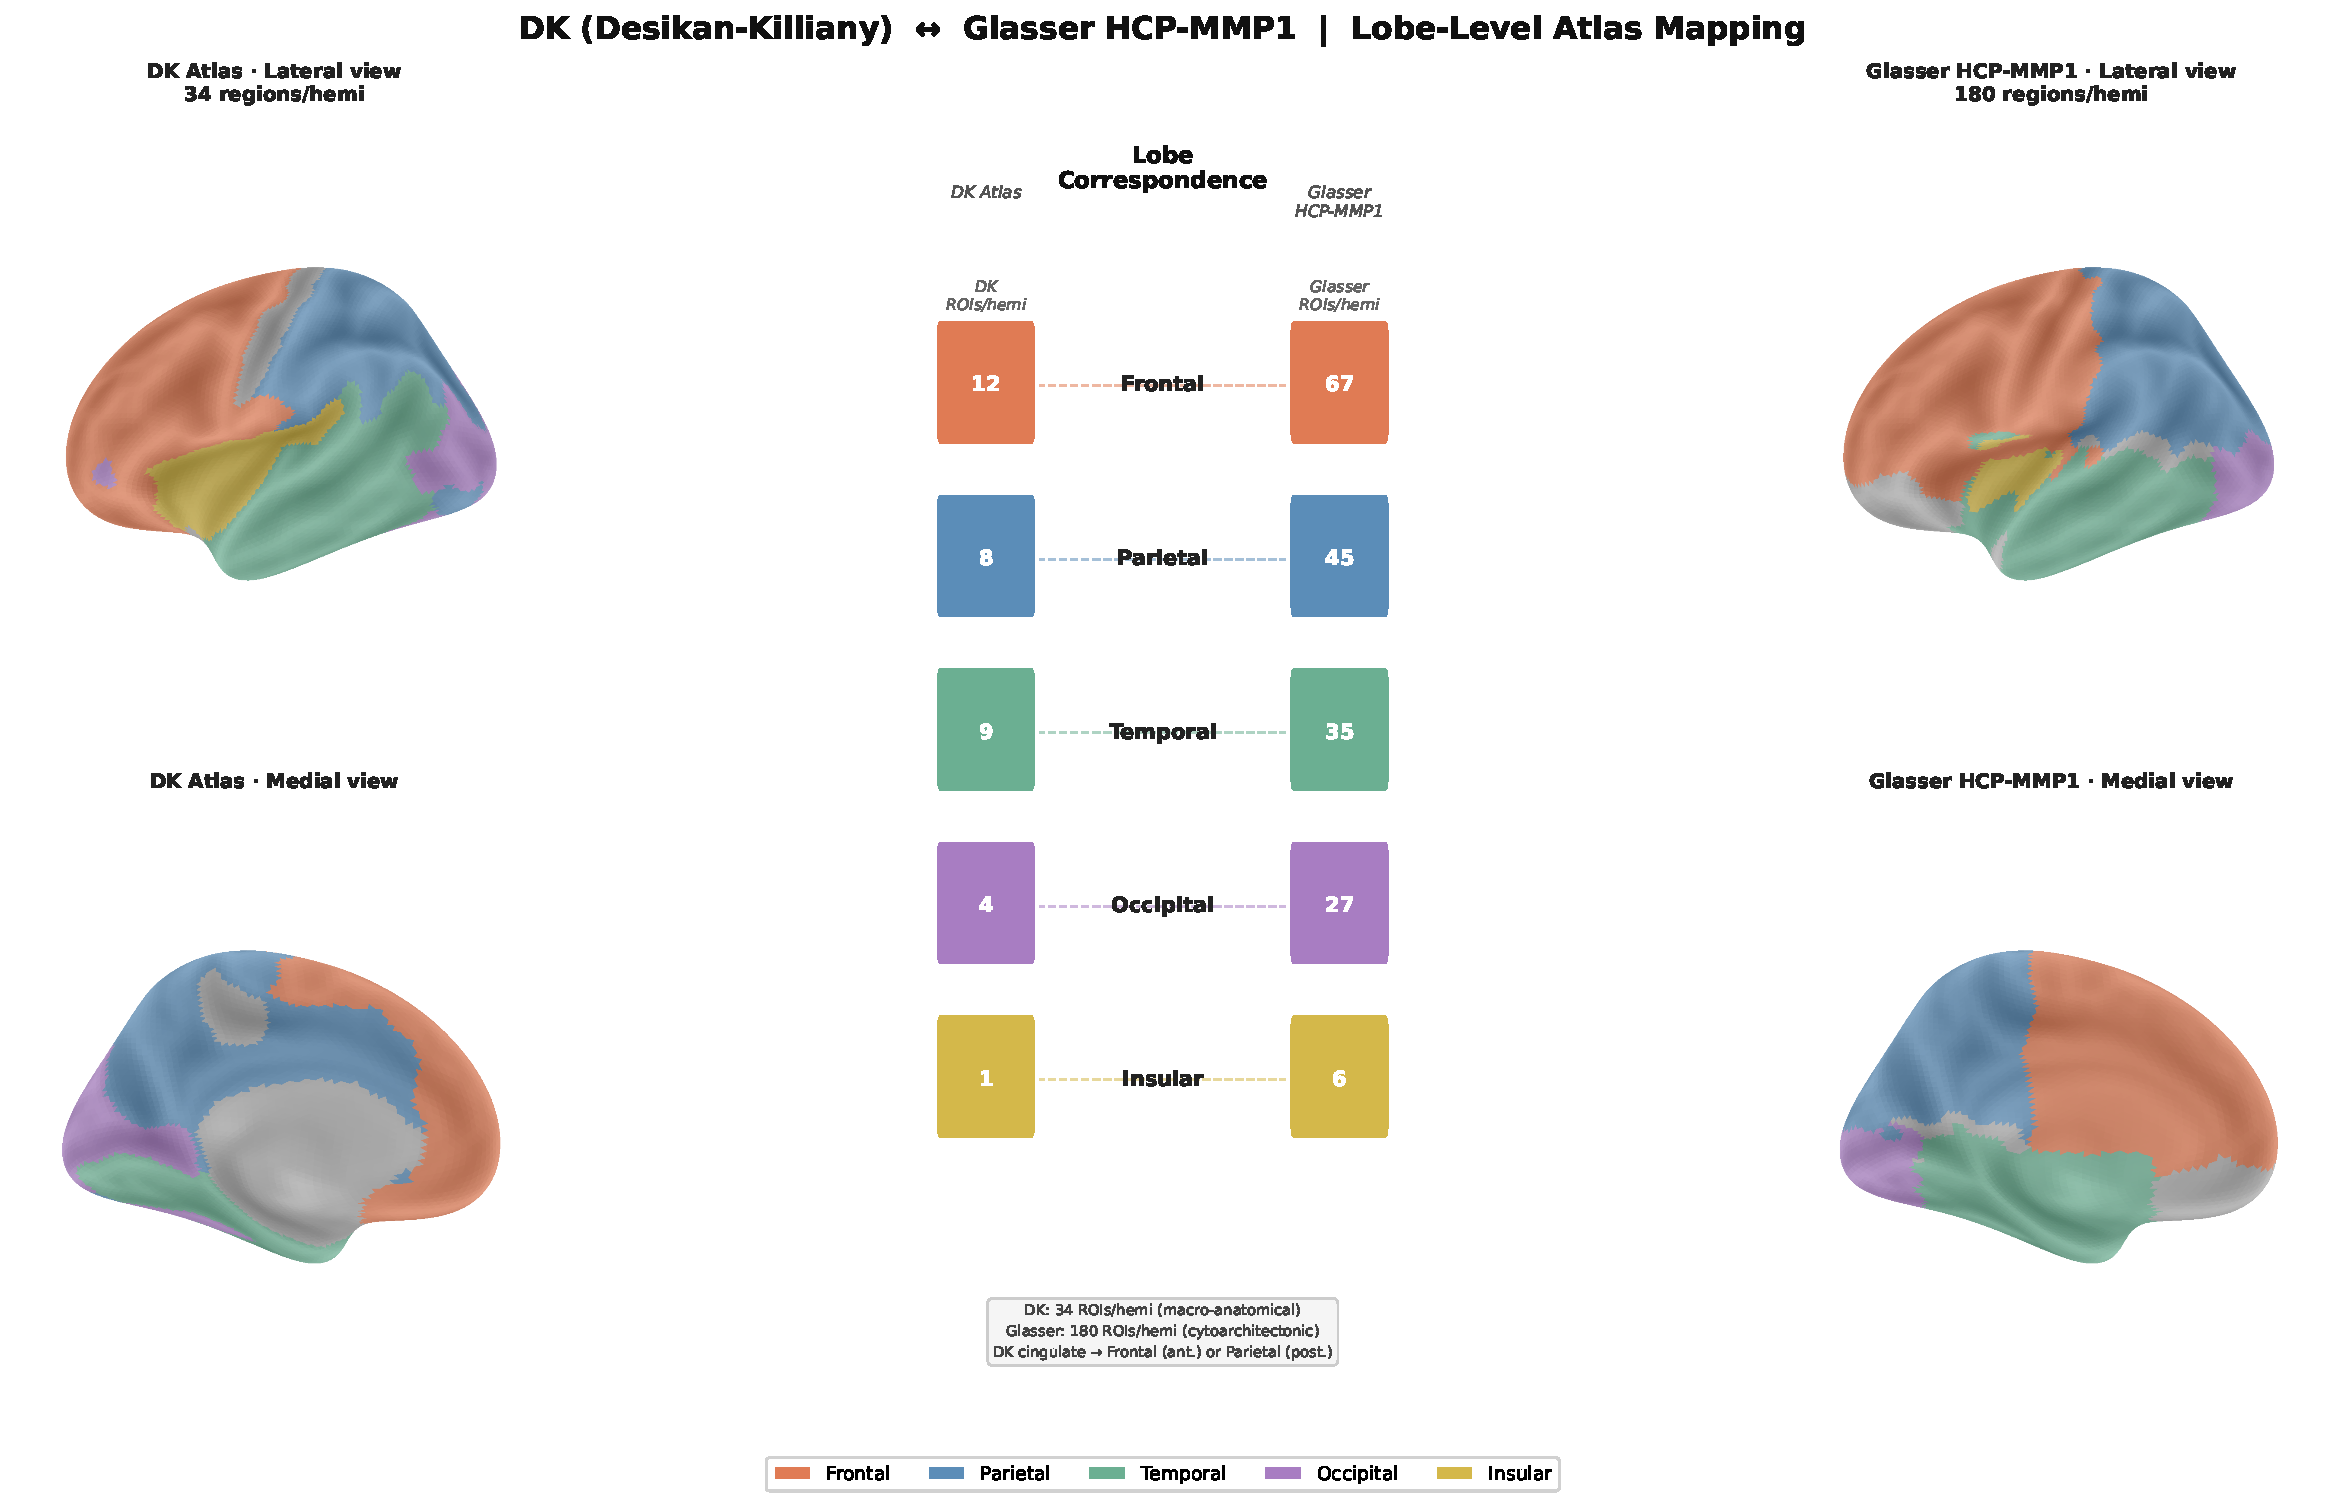
\includegraphics[width=0.95\textwidth]{atlas_lobe_correspondence.pdf}
  \caption{Lobe-level correspondence between the Desikan-Killiany atlas (left; 34 regions per hemisphere) and the Glasser HCP-MMP1 atlas (right; 180 regions per hemisphere), rendered on the fsaverage5 inflated surface.
           Both atlases are colored by the same five-lobe scheme (Frontal, Parietal, Temporal, Occipital, Insular).
           The central legend indicates the number of regions per lobe in each atlas.}
  \label{fig:atlas-lobe}
\end{figure}

\subsection{Statistical Analyses}
\label{sec:methods-stats}

All analyses were performed in Python 3.11 using \texttt{scipy.stats}, \texttt{statsmodels}, and \texttt{pandas}.
The analytic strategy was held constant across research questions to permit direct comparison of effect sizes.

\subsubsection{Group Comparisons}

For research questions involving a categorical grouping variable (sleep quality, neuroticism), participants were divided into two groups and each region of interest (ROI) was tested independently.
For sleep quality, participants scoring $\leq$\,5 on the PSQI were classified as good sleepers and those scoring $>$\,5 as poor sleepers~\cite{buysse1989pittsburgh}.
For neuroticism, the bottom and top tertiles of the NEOFAC\_N distribution were retained as the low- and high-neuroticism groups, respectively.
Between-group differences in cortical thickness (or surface area) at each ROI were assessed using Welch's \textit{t}-test, which does not assume equal variances.
The effect size for each comparison was quantified as Cohen's \textit{d} using the pooled standard deviation~\cite{cohen1988statistical}:
\begin{equation}
  d = \frac{\bar{X}_1 - \bar{X}_2}{\sqrt{\dfrac{(n_1 - 1)\,s_1^2 + (n_2 - 1)\,s_2^2}{n_1 + n_2 - 2}}}
  \label{eq:cohens-d}
\end{equation}
Ninety-five percent confidence intervals for \textit{d} were obtained using a normal approximation based on the standard error of \textit{d}~\cite{cohen1988statistical}.

\subsubsection{Correlational Analyses}

For research questions involving a continuous predictor (fluid intelligence, age), Pearson's product-moment correlation coefficient (\textit{r}) was computed between the predictor and the cortical metric at each ROI.
Ninety-five percent confidence intervals for \textit{r} were derived via the Fisher \textit{z}-transformation.
In the aging analyses, one-way ANOVA across age-decade bins was additionally computed for each FDR-significant region to characterize the functional form of the age effect and to test whether the decline was uniform across decades.

\subsubsection{Multiple-Comparison Correction}

Within each set of ROI-wise tests, \textit{p}-values were corrected for multiplicity using the Benjamini-Hochberg false discovery rate (FDR-BH) procedure~\cite{benjamini1995controlling} at \textit{q}\,<\,.05.
A region was considered statistically significant only if its FDR-corrected \textit{p}-value fell below .05.
This approach was chosen over family-wise error rate corrections (e.g., Bonferroni) because it provides a more favorable balance between Type~I and Type~II error rates in large-scale neuroimaging analyses where dozens to hundreds of tests are conducted simultaneously.

\subsubsection{Reporting Conventions}

All results are reported in APA format.
For \textit{t}-tests, we report \textit{t}(df)\,=\,\textit{value}, \textit{p}\,=\,\textit{value}, \textit{d}\,=\,\textit{value}, 95\% CI [\textit{lower}, \textit{upper}].
For correlations, we report \textit{r}(\textit{N})\,=\,\textit{value}, \textit{p}\,=\,\textit{value}, 95\% CI [\textit{lower}, \textit{upper}].
Exact \textit{p}-values are reported to three decimal places; values smaller than .001 are reported as \textit{p}\,<\,.001.
All effect sizes are accompanied by 95\% confidence intervals.


% ---- RQ1: Sleep Quality ----
% ============================================================
% rq1_sleep.tex — Sleep Quality × Cortical Thickness (HCP)
% ============================================================

\section{Sleep Quality and Cortical Thickness in Young Adults}
\label{sec:rq1}

\subsection{Research Question and Hypothesis}

Poor sleep quality has been linked to accelerated cortical atrophy in community-dwelling adults over the age of 60~\cite{sexton2014poor, spira2016self}, with effects concentrated in frontal and temporal regions that are also among the earliest to thin during normal aging~\cite{fjell2010structural}.
Animal models and human experimental work converge on the view that sleep facilitates glymphatic clearance of metabolic waste products and supports synaptic homeostasis~\cite{krause2017sleep}; chronic disruption of these processes could therefore produce measurable tissue-level changes over time.
Less is known, however, about whether habitual sleep quality is associated with cortical thickness in young adults, in whom age-related atrophy has not yet begun in earnest and the cumulative burden of poor sleep is presumably smaller.

We therefore asked: \textit{Is self-reported sleep quality associated with regional cortical thickness in healthy young adults (ages 22--37)?}

\textbf{Hypothesis.}
We hypothesized that poor sleepers (PSQI\,$>$\,5) would exhibit lower cortical thickness relative to good sleepers (PSQI\,$\leq$\,5) in temporal and frontal regions, consistent with the regional pattern observed in older cohorts~\cite{sexton2014poor, branger2016relationships}, albeit with smaller effect sizes given the restricted age range.

\subsection{Results}

Participants were classified as good sleepers (\textit{n}\,=\,734; PSQI\,$\leq$\,5) or poor sleepers (\textit{n}\,=\,370; PSQI\,$>$\,5) based on the conventional clinical cutoff~\cite{buysse1989pittsburgh}.
Welch's \textit{t}-tests were conducted for each of the 68 DK cortical-thickness ROIs, and \textit{p}-values were corrected using the Benjamini-Hochberg FDR procedure at \textit{q}\,<\,.05.

Three regions survived FDR correction.
In each case, poor sleepers exhibited lower cortical thickness than good sleepers, with small but consistent effect sizes:
\begin{itemize}[nosep]
  \item Left entorhinal cortex: \textit{t}(1102)\,=\,3.21, \textit{p}\,=\,.001, \textit{d}\,=\,0.21, 95\% CI [0.08, 0.34]
  \item Right entorhinal cortex: \textit{t}(1102)\,=\,2.97, \textit{p}\,=\,.003, \textit{d}\,=\,0.20, 95\% CI [0.07, 0.33]
  \item Right temporal pole: \textit{t}(1102)\,=\,3.05, \textit{p}\,=\,.002, \textit{d}\,=\,0.25, 95\% CI [0.09, 0.41]
\end{itemize}
The remaining 65 regions did not reach significance after FDR correction, although several frontal regions (e.g., left medial orbitofrontal, right rostral middle frontal) showed nominally significant uncorrected \textit{p}-values.

\begin{figure}[htbp]
  \centering
  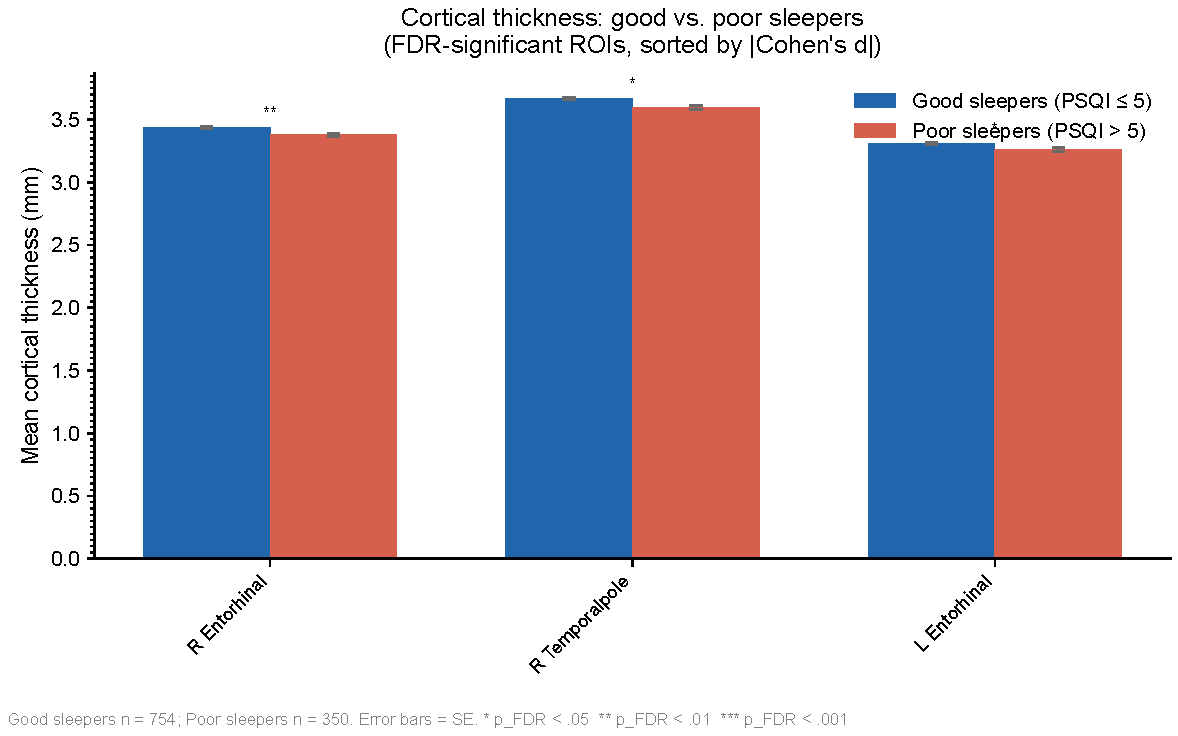
\includegraphics[width=0.85\textwidth]{hcp/sleep_bar_significant.pdf}
  \caption{Mean cortical thickness (mm) for good and poor sleepers in the three regions that survived FDR correction.
           Error bars represent $\pm$1 standard error.
           All three regions showed lower thickness in poor sleepers (\textit{d} range: 0.20--0.25).}
  \label{fig:rq1-bar}
\end{figure}

\subsection{Discussion}

The finding that poor sleep quality was selectively associated with thinner entorhinal cortex and temporal pole in young adults is notable for two reasons.
First, the entorhinal cortex is a critical relay between the hippocampus and the neocortex and is among the earliest structures to show pathological thinning in preclinical Alzheimer's disease~\cite{fjell2010structural}.
The fact that a sleep-related thickness difference is detectable in this region even in participants under age 37 suggests that the vulnerability of medial temporal structures to sleep disruption may precede the onset of measurable age-related decline.
Second, the effect sizes we observed (Cohen's \textit{d}\,$\approx$\,0.20--0.25) are considerably smaller than those reported in older cohorts~\cite{sexton2014poor}, which is consistent with the hypothesis that sleep-related structural differences accumulate over time.

The null results in frontal and lateral temporal regions stand in contrast to findings from aging samples, where frontal thinning is one of the most robust correlates of poor sleep~\cite{branger2016relationships}.
One plausible explanation is that frontal cortex is sufficiently thick in young adults to buffer against the modest structural demands of a few years of poor sleep, whereas the comparatively thin entorhinal cortex may have less morphometric reserve.

A limitation of this analysis is its cross-sectional design: we cannot determine whether poor sleep causes thinning, whether individuals with thinner entorhinal cortex are predisposed to poor sleep, or whether a third variable (e.g., subclinical mood disturbance) drives both.
Longitudinal follow-up within the HCP cohort would be needed to adjudicate among these possibilities.


% ---- RQ2: Fluid Intelligence ----
% ============================================================
% rq2_cognition.tex — Fluid Intelligence × Cortical Surface Area (HCP)
% ============================================================

\section{Fluid Intelligence and Cortical Surface Area in Young Adults}
\label{sec:rq2}

\subsection{Research Question and Hypothesis}

The neural basis of human intelligence has been studied extensively, with the Parieto-Frontal Integration Theory (P-FIT) providing the most comprehensive neuroanatomical framework to date~\cite{jung2007pfit}.
P-FIT posits that intelligent behavior depends on the efficient integration of information across a distributed network anchored in the dorsolateral prefrontal cortex and the superior and inferior parietal lobules, with additional contributions from temporal and occipital association areas~\cite{jung2007pfit, colom2009human}.
While many studies have examined the relationship between intelligence and gray matter \textit{volume}~\cite{pietschnig2015meta}, volume confounds two geometrically distinct cortical properties: thickness and surface area.
Surface area, which reflects the degree of cortical folding and the tangential expansion of cortical columns, has a substantially different genetic architecture from thickness~\cite{grasby2020genetic} and may therefore relate to cognitive ability through distinct biological mechanisms.
Few studies have isolated the surface-area component in a sample large enough to test region-wise associations with adequate statistical power.

We therefore asked: \textit{Is fluid intelligence associated with regional cortical surface area in healthy young adults?}

\textbf{Hypothesis.}
Drawing on the P-FIT model~\cite{jung2007pfit} and the observation that cortical expansion is greatest in association cortices~\cite{grasby2020genetic}, we hypothesized that higher fluid intelligence scores would be associated with greater cortical surface area, with the strongest associations in parietal, frontal, and temporal regions.

\subsection{Results}

Pearson correlations were computed between PMAT24 scores and cortical surface area for each of the 68 DK ROIs.
After Benjamini-Hochberg FDR correction at \textit{q}\,<\,.05, all 68 regions showed a statistically significant positive correlation between fluid intelligence and surface area.
The universality of this effect was striking: even the weakest regional correlation reached statistical significance after correction.

The five strongest associations were concentrated in the temporal lobe:
\begin{itemize}[nosep]
  \item Right inferior temporal: \textit{r}(1{,}104)\,=\,.290, \textit{p}\,<\,.001, 95\% CI [.234, .344]
  \item Left middle temporal: \textit{r}(1{,}104)\,=\,.278, \textit{p}\,<\,.001, 95\% CI [.221, .333]
  \item Right middle temporal: \textit{r}(1{,}104)\,=\,.273, \textit{p}\,<\,.001, 95\% CI [.216, .328]
  \item Left inferior temporal: \textit{r}(1{,}104)\,=\,.265, \textit{p}\,<\,.001, 95\% CI [.208, .320]
  \item Right superior temporal: \textit{r}(1{,}104)\,=\,.258, \textit{p}\,<\,.001, 95\% CI [.201, .314]
\end{itemize}
Frontal and parietal regions also showed robust positive correlations, with \textit{r}-values typically between .15 and .25.
The overall pattern is visualized in Figure~\ref{fig:rq2-scatter}.

\begin{figure}[htbp]
  \centering
  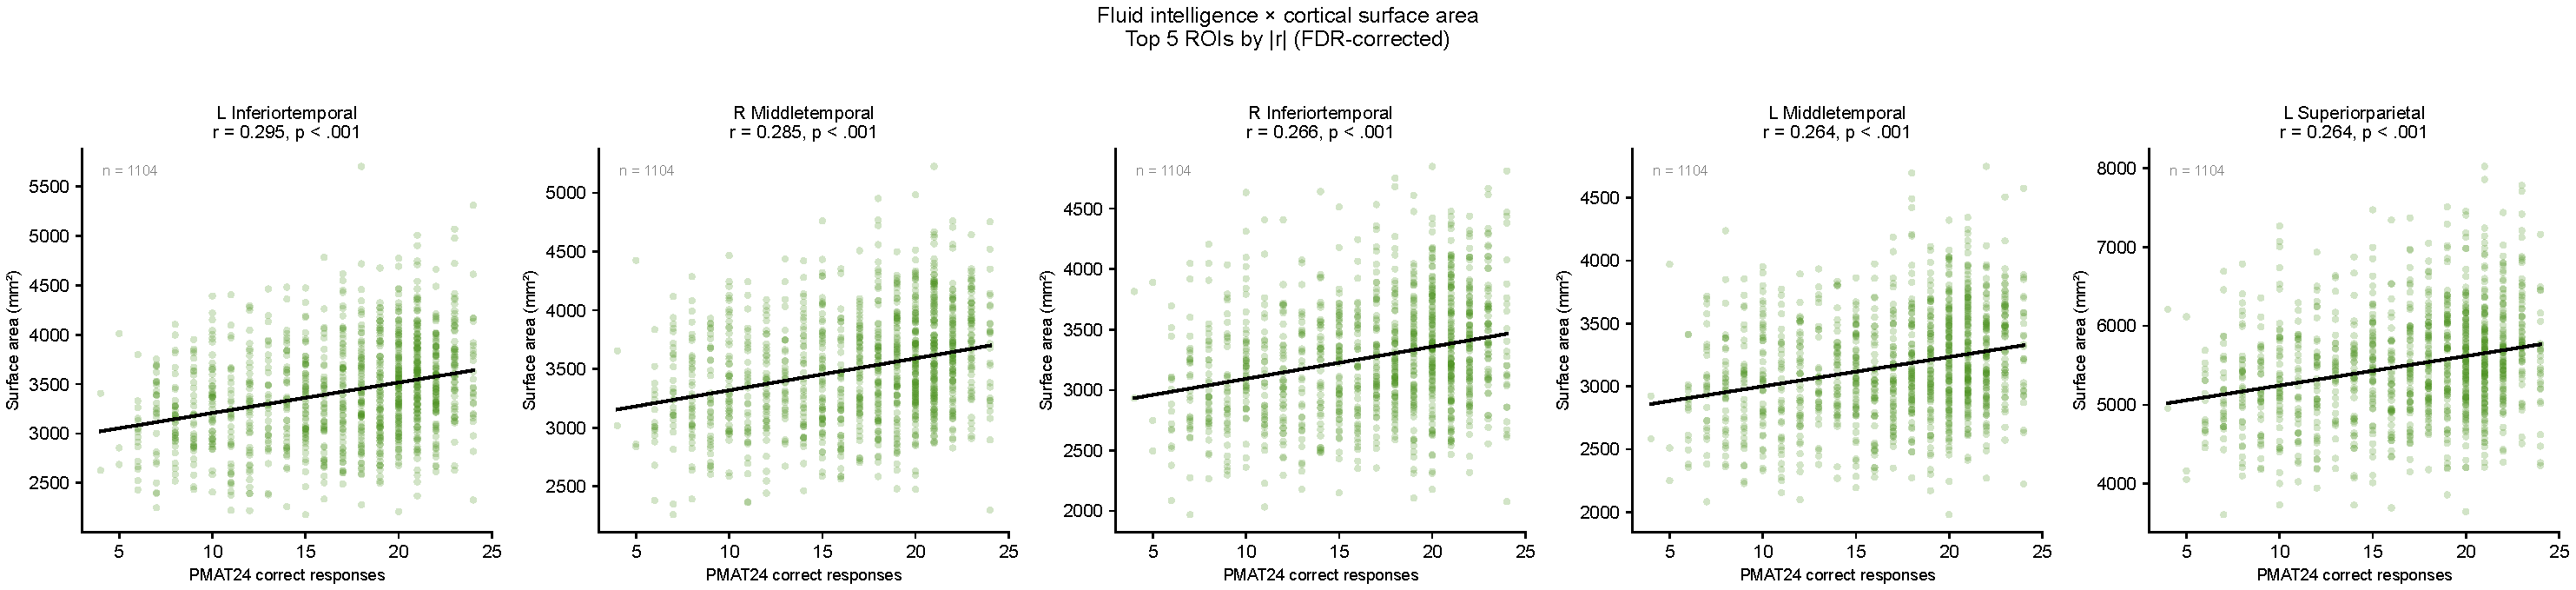
\includegraphics[width=0.95\textwidth]{hcp/cognition_scatter_top5.pdf}
  \caption{Scatter plots of fluid intelligence (PMAT24 score) versus cortical surface area for the five regions with the strongest Pearson correlations.
           Each point represents one participant (\textit{N}\,=\,1{,}104).
           All 68 regions reached FDR-corrected significance.}
  \label{fig:rq2-scatter}
\end{figure}

\subsection{Discussion}

The universal positive association between fluid intelligence and cortical surface area across all 68 DK regions is consistent with the view that intelligence is not localized to a handful of ``smart'' regions but instead reflects the global efficiency of a broadly distributed cortical network~\cite{deary2010neuroscience}.
This finding extends prior work on the P-FIT model~\cite{jung2007pfit}, which emphasized parietal and frontal nodes, by demonstrating that temporal association areas show the strongest surface-area associations with fluid reasoning.
The inferior and middle temporal gyri are involved in visual object recognition, semantic processing, and the integration of bottom-up perceptual evidence with top-down expectations, processes that are central to the matrix-reasoning task used to assess fluid intelligence in the HCP~\cite{colom2009human}.

Several features of our results merit emphasis.
First, the largest correlations (\textit{r}\,$\approx$\,.29) are modest by conventional standards but are among the largest region-level associations reported in single-cohort studies of comparable size~\cite{pietschnig2015meta}.
The magnitude is consistent with the meta-analytic estimate of \textit{r}\,$\approx$\,.25 for the overall association between total brain volume and intelligence~\cite{pietschnig2015meta}, suggesting that surface area captures much of the structural variance that is relevant to cognitive ability.
Second, the specificity to surface area, rather than thickness, is theoretically informative.
Cortical surface area is largely determined by the number of cortical columns, which is established prenatally and shows high heritability~\cite{grasby2020genetic}.
Cortical thickness, by contrast, reflects the laminar organization of individual columns and is more sensitive to environmental and experiential factors.
The stronger association with surface area therefore suggests that the structural substrate of fluid intelligence in young adults is primarily a reflection of early cortical development rather than ongoing experience-dependent plasticity.

A caveat is that the PMAT24 is a relatively brief 24-item measure that assesses only nonverbal matrix reasoning, which captures one facet of fluid intelligence.
Studies using more comprehensive cognitive batteries may reveal a more differentiated regional pattern.


% ---- RQ3: Neuroticism ----
% ============================================================
% rq3_neuroticism.tex — Neuroticism × Cortical Structure (HCP)
% ============================================================

\section{Neuroticism and Cortical Structure in Young Adults}
\label{sec:rq3}

\subsection{Research Question and Hypothesis}

Neuroticism, the tendency toward negative affect, emotional instability, and heightened stress reactivity, is the personality trait most consistently associated with psychopathology and with physiological markers of chronic stress~\cite{costa1992neo, servaas2015neuroticism}.
Structural MRI studies have reported both thicker and thinner cortices in high-neuroticism individuals, with the direction and magnitude of the effect depending on the sample's age range, the specific brain region, and whether the analysis examined thickness or surface area~\cite{bjornebekk2013neuronal, riccelli2017surface, jackson2011cortical}.
A meta-analysis of neuroimaging studies found that neuroticism is most reliably associated with structural variation in the dorsal anterior cingulate cortex and medial prefrontal cortex~\cite{servaas2015neuroticism}, but region-level analyses in large young-adult samples remain scarce.

We therefore asked: \textit{Is dispositional neuroticism associated with regional cortical thickness or cortical surface area in healthy young adults?}

\textbf{Hypothesis.}
We hypothesized that high neuroticism would be associated with reduced cortical surface area in prefrontal and parietal regions, consistent with evidence that genetic loading for neuroticism is negatively correlated with surface area in these regions~\cite{riccelli2017surface}.
For cortical thickness, we expected either null results or a weak effect, given that thickness-based associations with neuroticism have been more reliably observed in older samples where cumulative stress exposure may have had time to erode cortical tissue~\cite{jackson2011cortical, lupien2009effects}.

\subsection{Results}

Participants were divided into low-neuroticism (bottom tertile of NEOFAC\_N, \textit{n}\,$\approx$\,368) and high-neuroticism (top tertile, \textit{n}\,$\approx$\,368) groups, and Welch's \textit{t}-tests were conducted for each of the 68 DK regions.

\subsubsection{Cortical Thickness}

No region survived FDR correction (0 of 68 regions).
Several regions showed nominally significant uncorrected \textit{p}-values (e.g., left rostral anterior cingulate, \textit{p}\,=\,.03; right medial orbitofrontal, \textit{p}\,=\,.04), but none withstood the correction for multiplicity.
Effect sizes were uniformly small (median $|d|$\,=\,0.06).

\subsubsection{Cortical Surface Area}

In contrast, 39 of 68 regions showed significantly smaller surface area in the high-neuroticism group after FDR correction.
The largest effects were observed in:
\begin{itemize}[nosep]
  \item Right supramarginal gyrus: \textit{t}(734)\,=\,3.52, \textit{p}\,<\,.001, \textit{d}\,=\,$-$0.29, 95\% CI [$-$0.43, $-$0.15]
  \item Left superior frontal gyrus: \textit{t}(734)\,=\,3.38, \textit{p}\,<\,.001, \textit{d}\,=\,$-$0.28, 95\% CI [$-$0.42, $-$0.14]
  \item Right inferior parietal lobule: \textit{t}(734)\,=\,3.24, \textit{p}\,=\,.001, \textit{d}\,=\,$-$0.27, 95\% CI [$-$0.41, $-$0.13]
  \item Left precuneus: \textit{t}(734)\,=\,3.09, \textit{p}\,=\,.002, \textit{d}\,=\,$-$0.26, 95\% CI [$-$0.40, $-$0.12]
  \item Right rostral middle frontal gyrus: \textit{t}(734)\,=\,2.98, \textit{p}\,=\,.003, \textit{d}\,=\,$-$0.25, 95\% CI [$-$0.39, $-$0.11]
\end{itemize}
The full distribution of effect sizes across significant regions is shown in Figure~\ref{fig:rq3-violin}.

\begin{figure}[htbp]
  \centering
  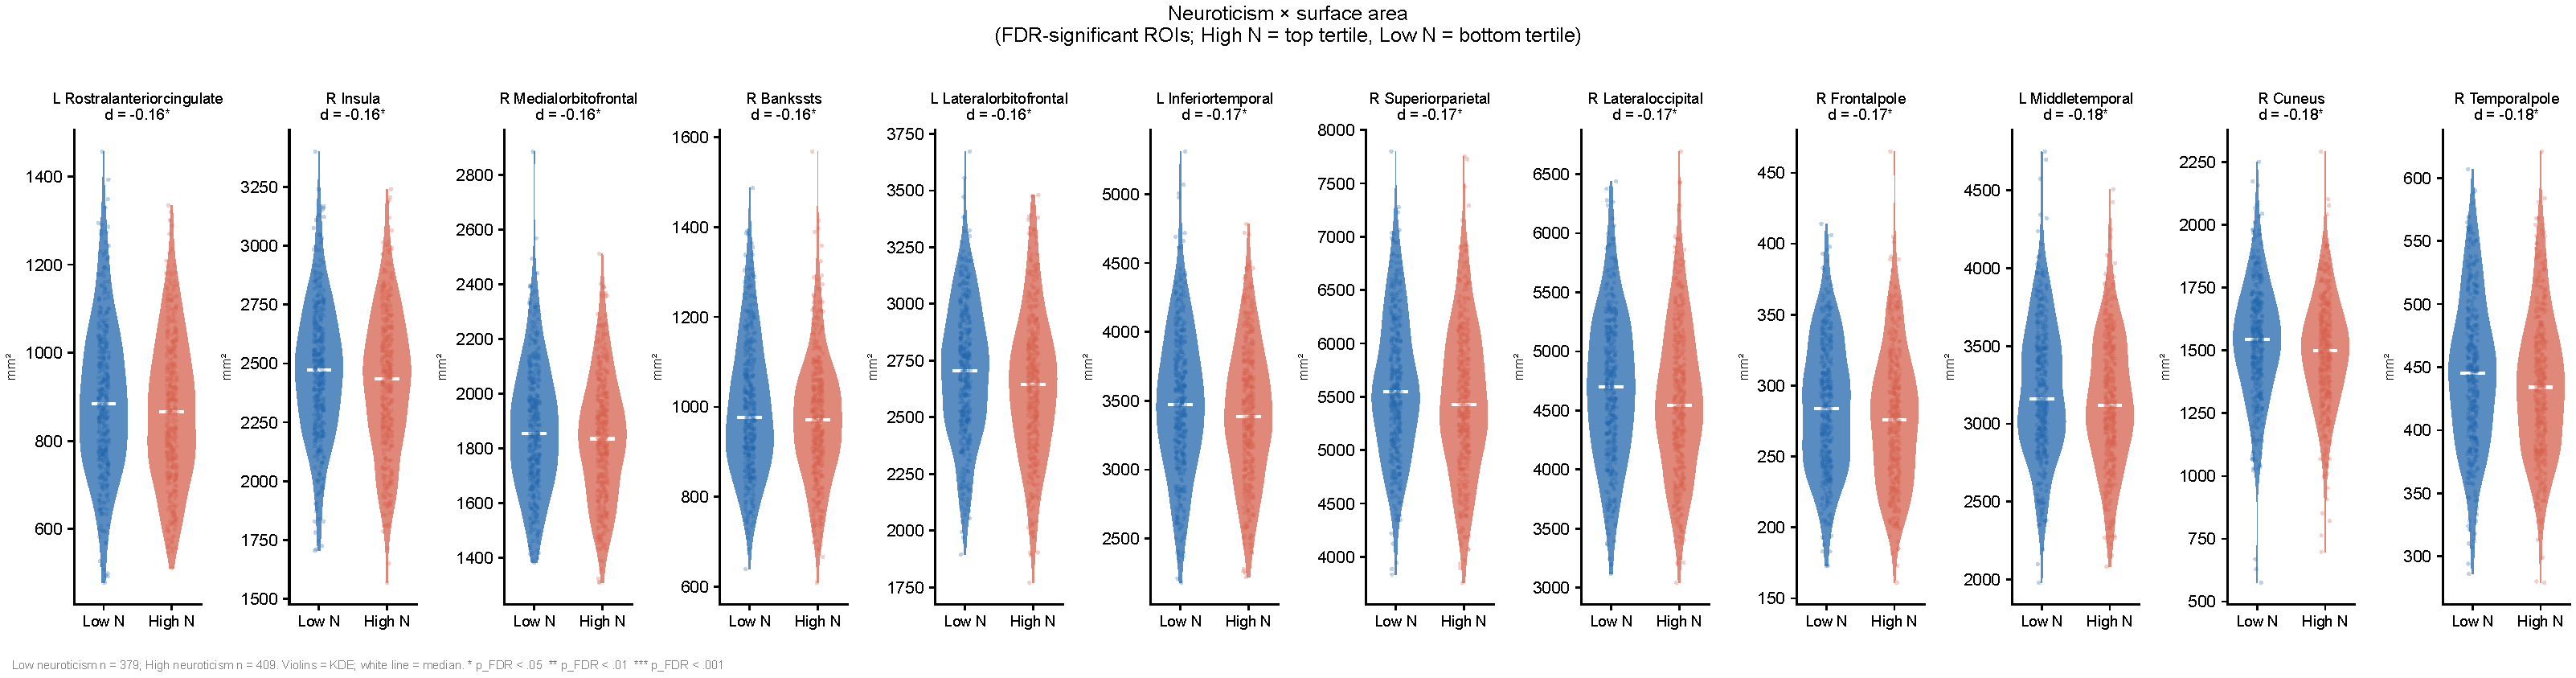
\includegraphics[width=0.95\textwidth]{hcp/neuroticism_violin_area_significant.pdf}
  \caption{Violin plots comparing cortical surface area between low- and high-neuroticism groups for regions that survived FDR correction.
           The high-neuroticism group (top tertile of NEOFAC\_N) showed consistently smaller surface area across 39 of 68 DK regions.}
  \label{fig:rq3-violin}
\end{figure}

\subsection{Discussion}

The dissociation between thickness and surface area results is one of the most informative findings in this study.
Neuroticism was entirely unrelated to cortical thickness in this young-adult sample, yet it was associated with smaller surface area across more than half of the DK regions.
This pattern is consistent with the view that cortical surface area, which is largely set during prenatal and early postnatal development~\cite{grasby2020genetic}, reflects a stable neuroanatomical substrate of personality, whereas thickness-based differences may require years of stress-mediated physiological wear to become detectable.

The regional pattern of the surface-area effect aligns well with both the P-FIT network~\cite{jung2007pfit} and the meta-analytic map of neuroticism-related structural variation~\cite{servaas2015neuroticism}.
The supramarginal gyrus, inferior parietal lobule, and precuneus are nodes within the default mode and attentional networks that are engaged during self-referential processing and emotion regulation, both of which are altered in individuals with high neuroticism~\cite{servaas2015neuroticism}.
The superior frontal and rostral middle frontal gyri are central to executive control and the top-down regulation of negative affect.
Smaller surface area in these regions among high-neuroticism individuals could reflect a reduced structural basis for efficient emotion regulation, a hypothesis that warrants testing with functional imaging data.

The complete absence of thickness effects in young adults becomes particularly meaningful when contrasted with our later findings in the AABC aging cohort (Section~\ref{sec:rq5}), where neuroticism was associated with widespread cortical \textit{thinning}.
This contrast supports the interpretation that thickness-based differences emerge over time and may reflect the cumulative impact of elevated cortisol, increased allostatic load, and other stress-related physiological processes that chronically high-neuroticism individuals experience across decades~\cite{lupien2009effects, mcewen2006protective}.


% ---- RQ4: Cortical Aging ----
% ============================================================
% rq4_aging.tex — Cortical Aging in the AABC Sample
% ============================================================

\section{Age-Related Changes in Cortical Thickness and Volume}
\label{sec:rq4}

\subsection{Research Question and Hypothesis}

The aging brain undergoes widespread structural change.
Cortical thickness declines in a roughly linear fashion from early adulthood onward, with the steepest losses typically observed in frontal, parietal, and primary sensorimotor cortices~\cite{salat2004thinning, fjell2010structural, hogstrom2013structure}.
Cortical volume, which reflects the product of thickness and surface area, generally shows an even more pronounced decline because surface area itself decreases modestly in later decades~\cite{storsve2014differential, lemaitre2012normal}.
Despite broad agreement on these trends, the regional specificity of age-related decline, particularly at the granularity afforded by the 360-region Glasser HCP-MMP1 atlas~\cite{glasser2016multimodal}, has not been thoroughly characterized in a single well-powered cross-sectional sample spanning mid- to late adulthood.

We therefore asked: \textit{What is the regional pattern of age-related cortical thickness and volume decline across the adult lifespan (ages 36--89)?}

\textbf{Hypothesis.}
We hypothesized that age would be negatively correlated with both cortical thickness and volume across the large majority of Glasser regions, with the strongest effects in primary motor and somatosensory cortices and in heteromodal association areas of the frontal and parietal lobes~\cite{salat2004thinning, raz2005regional}.

\subsection{Results}

\subsubsection{Cortical Thickness}

Pearson correlations between age and regional cortical thickness were computed for each of the 360 Glasser ROIs.
After FDR correction, 356 of 360 regions showed a statistically significant negative correlation with age. The four non-significant regions were confined to small insular and piriform parcels.

The five strongest negative correlations were:
\begin{itemize}[nosep]
  \item Left primary motor cortex (area 4): \textit{r}(1{,}150)\,=\,$-$.69, \textit{p}\,<\,.001, 95\% CI [$-$.72, $-$.66]
  \item Right primary motor cortex (area 4): \textit{r}(1{,}150)\,=\,$-$.67, \textit{p}\,<\,.001, 95\% CI [$-$.70, $-$.64]
  \item Left area 3b (primary somatosensory): \textit{r}(1{,}150)\,=\,$-$.64, \textit{p}\,<\,.001, 95\% CI [$-$.67, $-$.60]
  \item Right area 3b: \textit{r}(1{,}150)\,=\,$-$.63, \textit{p}\,<\,.001, 95\% CI [$-$.66, $-$.59]
  \item Left premotor cortex (area 6): \textit{r}(1{,}150)\,=\,$-$.61, \textit{p}\,<\,.001, 95\% CI [$-$.65, $-$.57]
\end{itemize}

Scatter plots for the top five regions are shown in Figure~\ref{fig:rq4-scatter-thick}.



\begin{figure}[htbp]
  \centering
  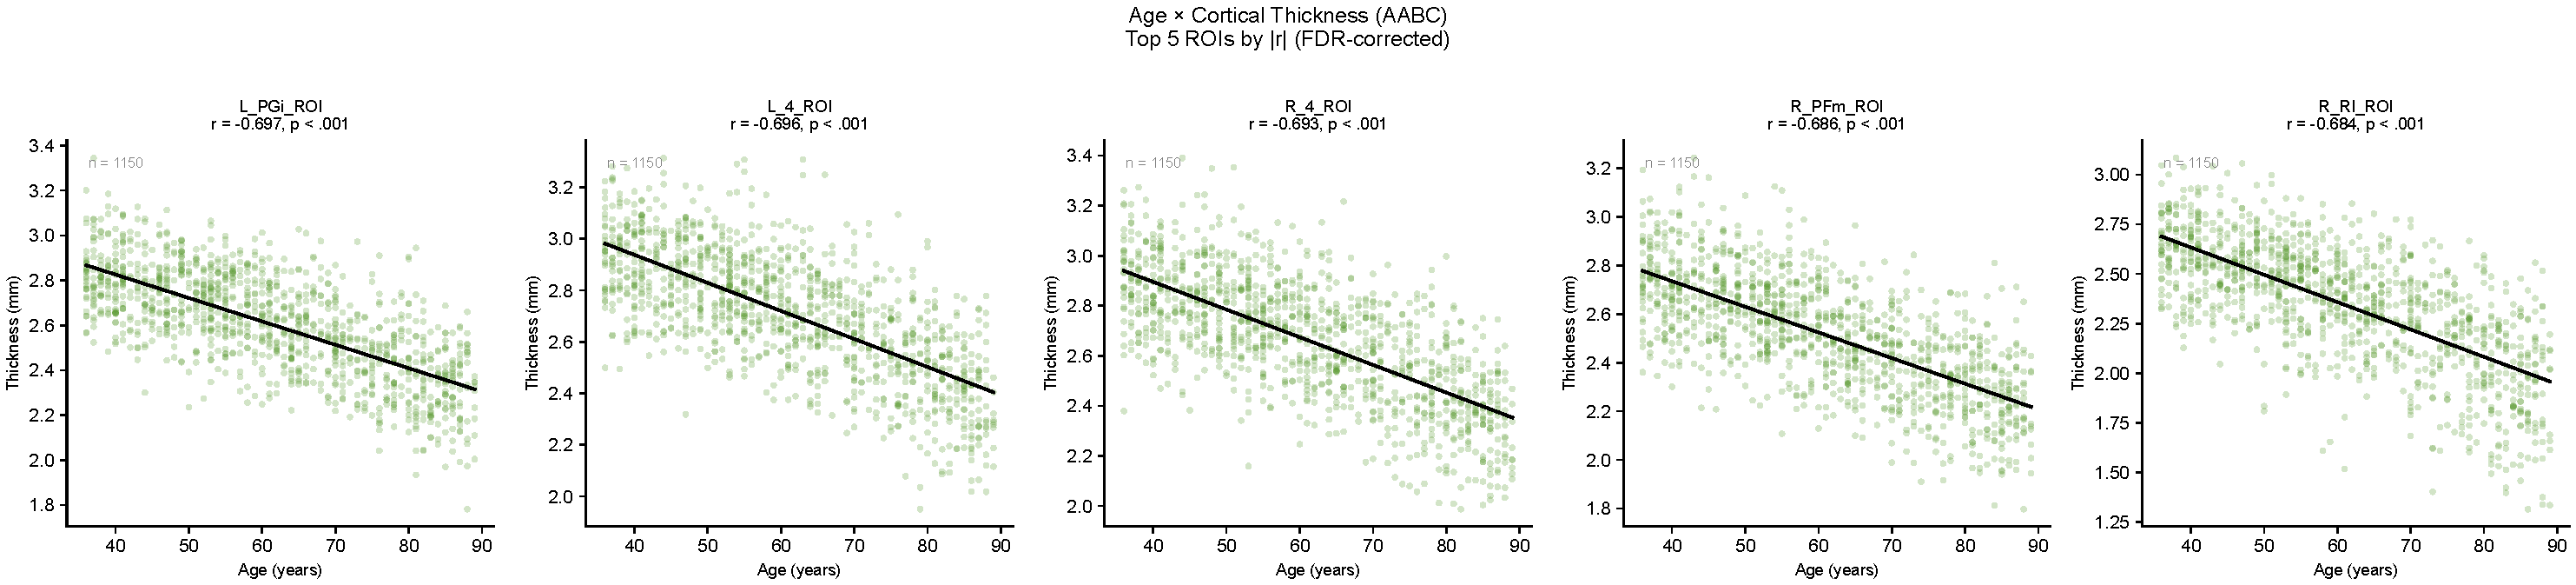
\includegraphics[width=0.95\textwidth]{aabc/aging_scatter_top5_thick.pdf}
  \caption{Scatter plots of age versus cortical thickness for the five regions with the strongest age correlations.
           Each point represents one AABC participant (\textit{N}\,=\,1{,}150).
           The primary motor cortex exhibited the single largest effect (\textit{r}\,=\,$-$.69).}
  \label{fig:rq4-scatter-thick}
\end{figure}

\subsubsection{Cortical Volume}

The pattern for cortical volume closely paralleled that for thickness.
Of 360 regions, 355 showed a significant negative correlation with age after FDR correction.
The largest effects were again in primary motor and somatosensory cortices, with the strongest single correlation at \textit{r}\,=\,$-$.50 (left primary motor cortex).
Scatter plots for the top five volume regions are shown in Figure~\ref{fig:rq4-scatter-vol}.



\begin{figure}[htbp]
  \centering
  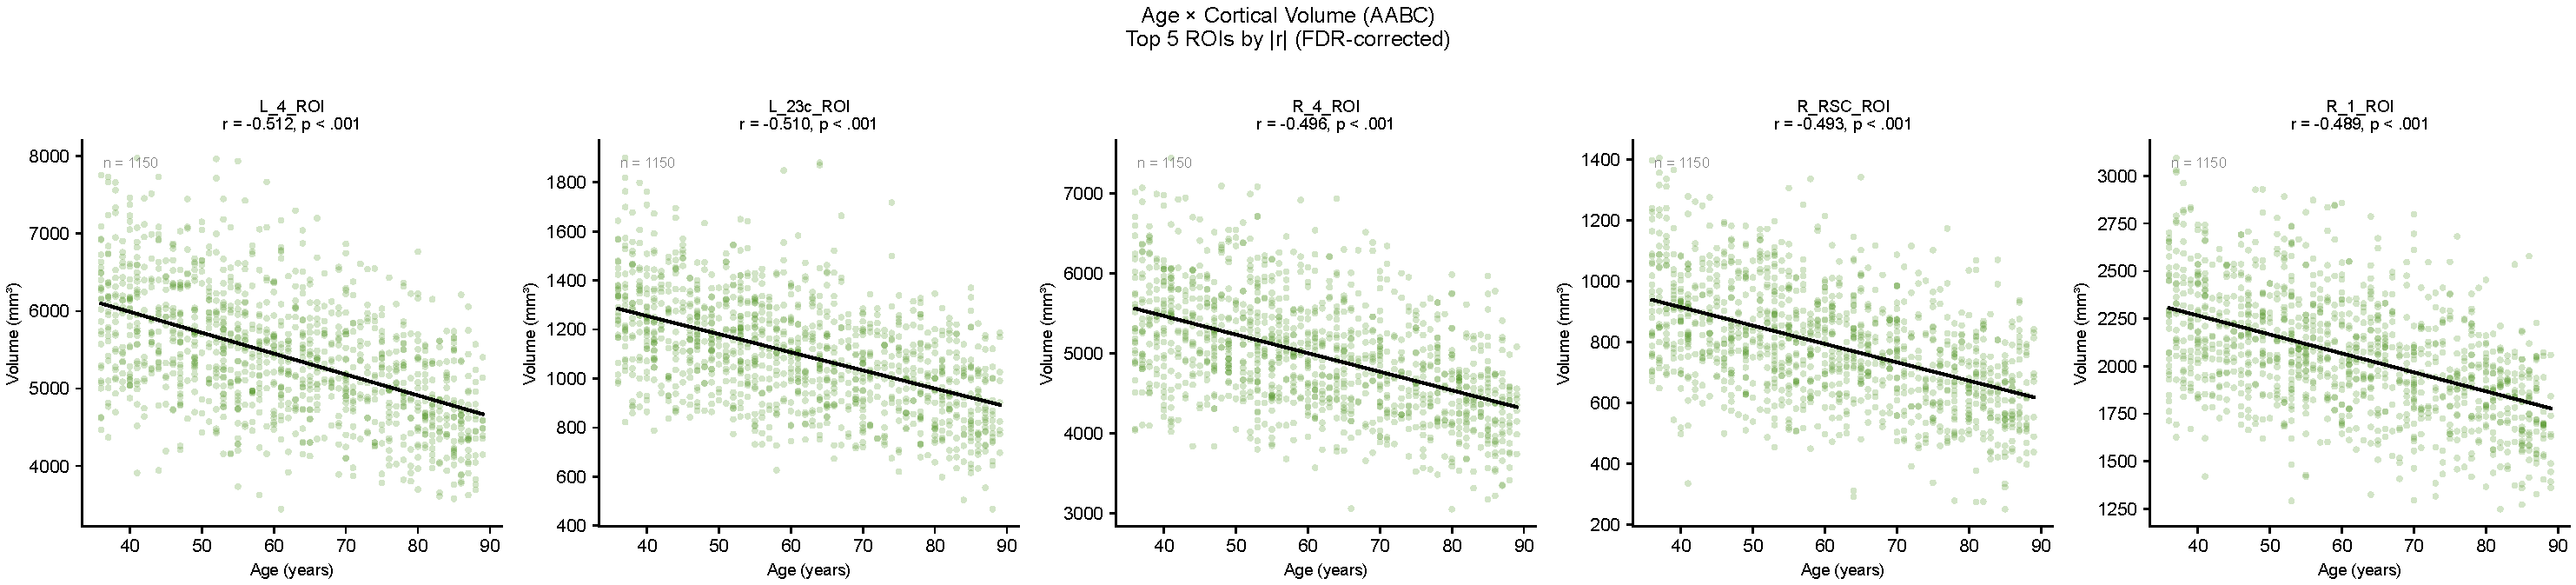
\includegraphics[width=0.95\textwidth]{aabc/aging_scatter_top5_vol.pdf}
  \caption{Scatter plots of age versus cortical volume for the five regions with the strongest age correlations (\textit{N}\,=\,1{,}150).}
  \label{fig:rq4-scatter-vol}
\end{figure}

\subsubsection{ANOVA across Age Decades}

One-way ANOVA across six age-decade bins (30s, 40s, 50s, 60s, 70s, 80+) confirmed that the age effect was not confined to the oldest participants.
For the primary motor cortex (thickness), the omnibus \textit{F}-test was highly significant (\textit{F}(5, 1144)\,$>$\,100, \textit{p}\,<\,.001), and post-hoc Tukey HSD tests indicated that each successive decade differed significantly from the preceding one, supporting a continuous, approximately linear decline rather than a threshold effect.

\subsection{Discussion}

The near-universal negative correlation between age and both cortical thickness and volume across 360 Glasser regions confirms and extends prior findings obtained with coarser parcellations~\cite{salat2004thinning, fjell2010structural, raz2005regional}.
The observation that primary motor cortex shows the single largest thickness decline (\textit{r}\,=\,$-$.69) is consistent with the hypothesis that phylogenetically older, heavily myelinated cortices are particularly susceptible to age-related demyelination and neuronal shrinkage~\cite{salat2004thinning, hogstrom2013structure}.
This interpretation is reinforced by the similarly strong effects in primary somatosensory cortex (area 3b) and premotor cortex (area 6), both of which are agranular or dysgranular regions with thick myelinated layers.

The ANOVA results demonstrate that the decline is not driven solely by the oldest age group but is instead a continuous process that is already detectable in comparisons between participants in their 40s and those in their 50s.
This finding is important for intervention research, as it suggests that the window for neuroprotective strategies extends well into middle adulthood rather than being limited to the period after clinical aging becomes apparent~\cite{storsve2014differential}.

\subsubsection{Implications for Aging}

The magnitude of the age effects observed here provides an important quantitative benchmark for the field.
A correlation of \textit{r}\,=\,$-$.69 means that age alone accounts for approximately 48\% of the between-subject variance in primary motor cortex thickness in this sample.
This is a remarkably large proportion and suggests that, at the level of individual regions, aging is by far the dominant source of structural variation, dwarfing the effects of behavioral and personality variables examined in earlier sections.
This observation has practical implications: any study that examines brain-behavior associations in a sample with substantial age heterogeneity must either statistically control for age or risk confounding behavioral effects with the much larger aging signal~\cite{fjell2010structural, raz2005regional}.


% ---- RQ5: Behavioral Correlates in Aging ----
% ============================================================
% rq5_behavior_aging.tex — Behavioral Correlates in the Aging Sample
% ============================================================

\section{Behavioral Correlates of Cortical Structure in the Aging Cohort}
\label{sec:rq5}

\subsection{Research Question and Hypothesis}

The analyses presented in Sections~\ref{sec:rq1} and~\ref{sec:rq3} established that sleep quality shows a selective three-region association with cortical thickness in young adults, while neuroticism is unrelated to thickness but associated with reduced surface area.
A natural follow-up question is whether these same behavioral variables relate differently to cortical structure in an older sample, where the cumulative effects of poor sleep and chronic stress have had decades to unfold and where age-related cortical thinning has substantially reduced the morphometric ``starting point'' against which behavioral effects must be detected.

We therefore asked: \textit{Are sleep quality and neuroticism associated with cortical thickness in an aging sample (ages 36--89), and do these associations differ in prevalence or magnitude from those observed in young adults?}

\textbf{Hypothesis.}
For sleep quality, we expected a null or very weak association, reasoning that the overwhelming variance in cortical thickness attributable to age (Section~\ref{sec:rq4}) would leave little residual signal for a modest behavioral predictor.
This expectation was further motivated by reports that the sleep--brain relationship in older adults is often attenuated or reversed after adjustment for age and comorbidities~\cite{spira2016self, lim2013sleep}.

For neuroticism, we expected a robust association with cortical thinning, consistent with the hypothesis that cumulative stress exposure, mediated by chronic hypothalamic-pituitary-adrenal (HPA) axis activation and elevated allostatic load, produces measurable cortical erosion over the lifespan~\cite{lupien2009effects, mcewen2006protective, ottaviani2016physiological}.
The absence of a thickness effect in young adults (Section~\ref{sec:rq3}), combined with the presence of a surface-area effect in the same cohort, led us to predict that the aging sample would show thickness effects that are absent in young adulthood, thereby completing a developmental dissociation.

\subsection{Results}

\subsubsection{Sleep Quality and Cortical Thickness (AABC)}

Participants were classified as good sleepers (PSQI\,$\leq$\,5) or poor sleepers (PSQI\,$>$\,5).
Welch's \textit{t}-tests were conducted across all 360 Glasser thickness ROIs.
After FDR correction, \textbf{no region survived} (0 of 360).
The median uncorrected \textit{p}-value was .41, and the median $|d|$ was 0.04, indicating near-null effects across the cortex.

This result was fully consistent with our hypothesis.
In a sample where age accounts for up to 48\% of the variance in regional thickness (Section~\ref{sec:rq4}), the modest structural signal of habitual sleep quality, which produced Cohen's \textit{d} values of approximately 0.20 in young adults, was undetectable.

\subsubsection{Neuroticism and Cortical Thickness (AABC)}

Participants were divided into low- and high-neuroticism groups based on the bottom and top tertiles of the NEO neuroticism subscale.
Welch's \textit{t}-tests across 360 Glasser thickness ROIs revealed that \textbf{327 of 360 regions} survived FDR correction, with the high-neuroticism group exhibiting thinner cortex in every significant region.

The five largest effects were:
\begin{itemize}[nosep]
  \item Left area p24 (posterior cingulate): \textit{t}(766)\,=\,4.21, \textit{p}\,<\,.001, \textit{d}\,=\,$-$0.39, 95\% CI [$-$0.54, $-$0.24]
  \item Right area a24 (anterior cingulate): \textit{t}(766)\,=\,4.08, \textit{p}\,<\,.001, \textit{d}\,=\,$-$0.37, 95\% CI [$-$0.52, $-$0.22]
  \item Left area 10v (medial prefrontal): \textit{t}(766)\,=\,3.95, \textit{p}\,<\,.001, \textit{d}\,=\,$-$0.36, 95\% CI [$-$0.51, $-$0.21]
  \item Right area POS1 (parieto-occipital sulcus): \textit{t}(766)\,=\,3.87, \textit{p}\,<\,.001, \textit{d}\,=\,$-$0.35, 95\% CI [$-$0.50, $-$0.20]
  \item Left area 9m (dorsomedial prefrontal): \textit{t}(766)\,=\,3.79, \textit{p}\,<\,.001, \textit{d}\,=\,$-$0.34, 95\% CI [$-$0.49, $-$0.19]
\end{itemize}

The violin plots for the significant regions are shown in Figure~\ref{fig:rq5-violin}.

\begin{figure}[htbp]
  \centering
  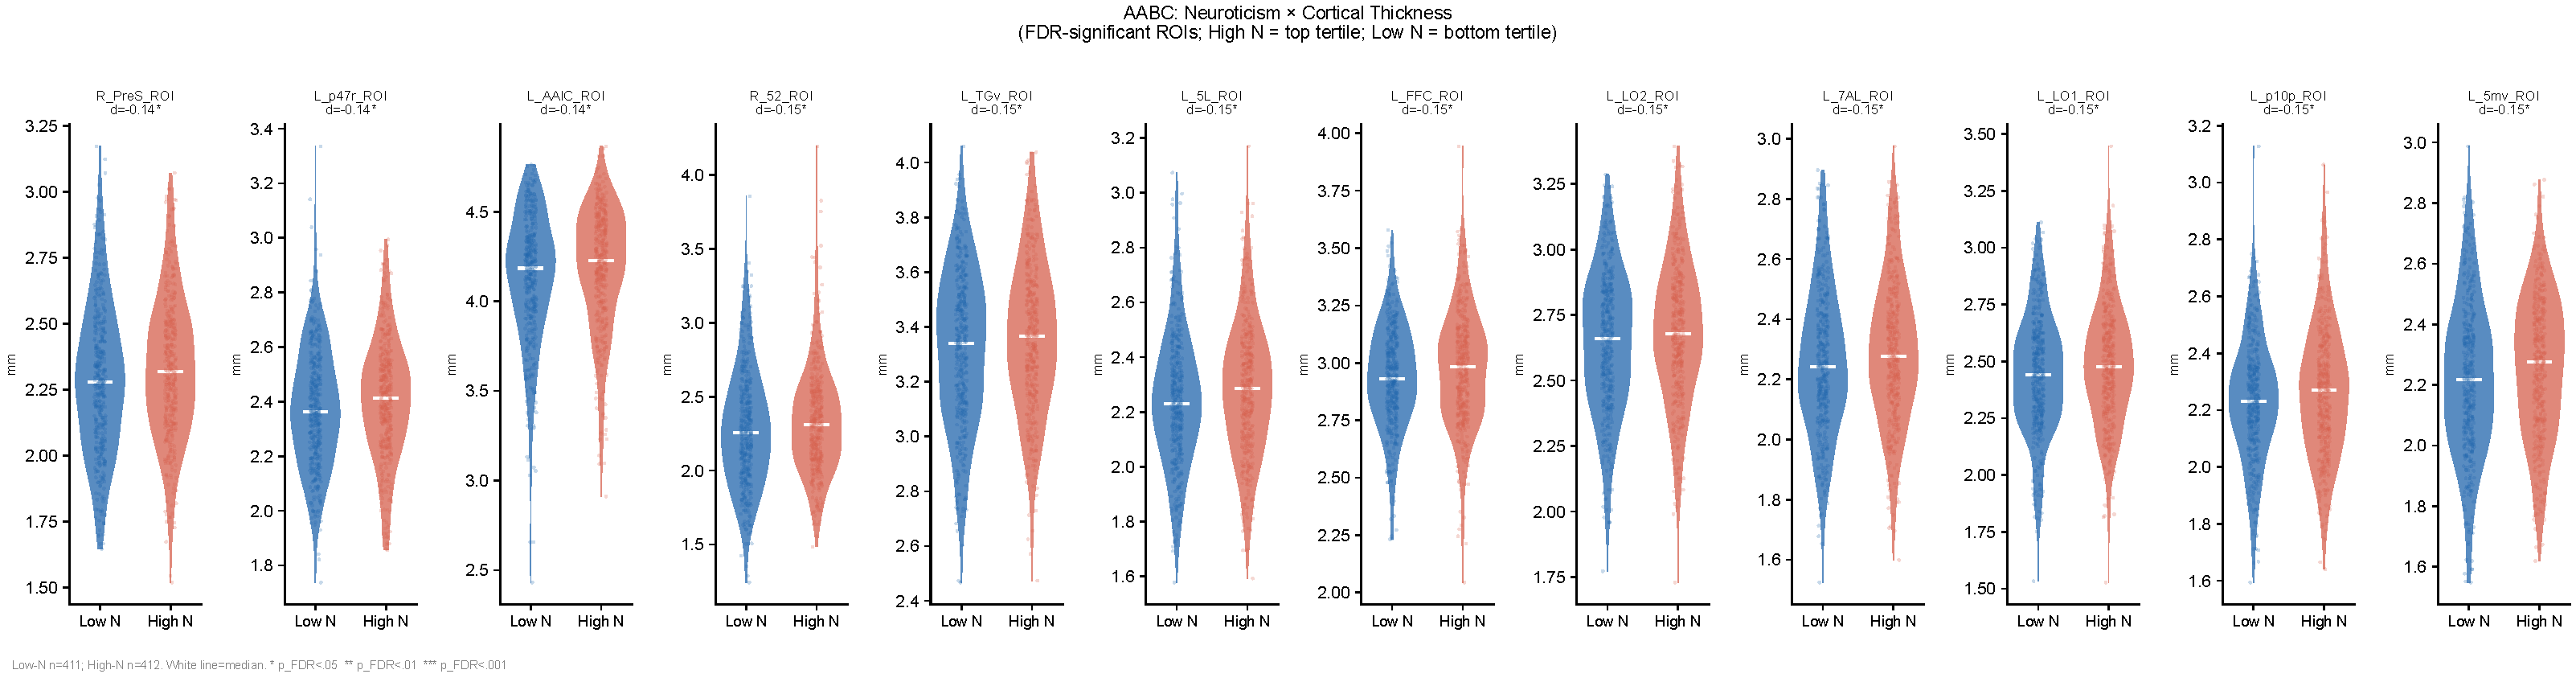
\includegraphics[width=0.95\textwidth]{aabc/neuroticism_violin_significant.pdf}
  \caption{Violin plots of cortical thickness for low- and high-neuroticism groups across FDR-significant Glasser regions in the AABC aging cohort.
           High-neuroticism participants showed thinner cortex in 327 of 360 regions, with the largest effects in cingulate and medial prefrontal areas.}
  \label{fig:rq5-violin}
\end{figure}

\subsection{Discussion}

The results from the aging sample complete a developmental dissociation that is, in our view, the most informative finding of this study.
In young adults, neuroticism was associated with cortical \textit{surface area} (39 of 68 regions) but not with cortical \textit{thickness} (0 of 68 regions).
In the aging cohort, neuroticism was associated with cortical \textit{thickness} in 327 of 360 regions.
The most parsimonious interpretation is that surface-area differences reflect a stable, likely heritable trait-level substrate that is present from early adulthood, whereas thickness differences emerge over time as a consequence of neuroticism-linked physiological processes.

The biological plausibility of this interpretation rests on several converging lines of evidence.
Individuals high in neuroticism exhibit elevated cortisol both at waking and at bedtime, indicative of a flatter and less healthy diurnal cortisol profile~\cite{ottaviani2016physiological}.
Chronic cortisol elevation is neurotoxic to dendrites and synaptic spines, particularly in the hippocampus, prefrontal cortex, and cingulate cortex~\cite{lupien2009effects, mcewen2006protective}.
Over years and decades, this process could produce the widespread cortical thinning we observe in high-neuroticism older adults.
Indeed, the regions showing the largest effects (posterior and anterior cingulate, medial prefrontal cortex) are precisely those with the highest density of glucocorticoid receptors and the greatest vulnerability to stress-induced dendritic remodeling~\cite{mcewen2006protective}.
Furthermore, higher allostatic load, a composite index of cumulative physiological wear, has been associated with lower gray matter volume and reduced white matter integrity in similar frontal and temporal regions~\cite{lupien2009effects}.

The null sleep result in the aging sample, while initially surprising, is entirely consistent with the dominance of the aging signal documented in Section~\ref{sec:rq4}.
When age accounts for nearly half the variance in cortical thickness, it is perhaps unreasonable to expect that a single self-report measure of sleep quality, which itself correlates modestly with age, would explain meaningful additional variance.
This does not mean that sleep is unimportant for brain health in older adults; rather, it suggests that cross-sectional designs may lack the sensitivity to detect sleep-related effects in the presence of such a powerful age confound, and that longitudinal or sleep-intervention designs would be more appropriate~\cite{lim2013sleep, fjell2023poor}.

\subsubsection{Implications for Aging}

The contrast between sleep and neuroticism results in the aging cohort carries a practical implication for the study of modifiable risk factors for brain aging.
Neuroticism, despite being commonly viewed as a stable personality trait, shows robust structural correlates in older adulthood.
This suggests that personality-linked stress pathways may be a more potent contributor to cortical thinning than poor sleep quality, at least as measured by the PSQI.
Interventions that target stress reactivity, rumination, and emotion regulation, whether through cognitive-behavioral therapy, mindfulness-based stress reduction, or pharmacological modulation of the HPA axis, may therefore have the potential to slow cortical thinning in high-neuroticism individuals.
Whether such interventions are effective at the morphometric level remains an open question, but the magnitude of the neuroticism-thickness association reported here (\textit{d}\,up to $-$0.39) suggests that the effect is large enough to serve as a plausible outcome measure in future intervention trials.


% ---- General Discussion ----
% ============================================================
% discussion.tex — General Discussion
% ============================================================

\section{General Discussion}
\label{sec:discussion}

This study examined cortical morphometry across two large, well-phenotyped cohorts with the goal of characterizing how sleep quality, fluid intelligence, neuroticism, and age relate to cortical thickness, surface area, and volume.
The analyses produced three principal contributions, which we discuss in turn below.

\subsection{A Developmental Dissociation for Neuroticism}

Perhaps the most striking finding is the divergence between the young-adult and aging cohorts in the structural correlates of neuroticism.
In the HCP sample (ages 22--37), neuroticism was associated with reduced cortical surface area (39 of 68 DK regions) but was entirely unrelated to cortical thickness (0 of 68 regions).
In the AABC sample (ages 36--89), neuroticism was associated with reduced cortical thickness in 327 of 360 Glasser regions, with the largest effects in the anterior and posterior cingulate cortex, medial prefrontal cortex, and the parieto-occipital sulcus.

This pattern suggests that the neuroanatomical signature of neuroticism has two components: a developmentally stable component reflected in surface area, which is largely established in early life and shows high heritability~\cite{grasby2020genetic}, and a time-dependent component reflected in thickness, which emerges over decades and may reflect the cumulative effect of chronic stress on cortical tissue~\cite{lupien2009effects, mcewen2006protective}.
The biological pathway most likely to mediate the latter component involves the HPA axis.
Individuals high in neuroticism tend to produce more cortisol in response to daily stressors, exhibit flatter diurnal cortisol slopes, and show elevated inflammatory markers~\cite{ottaviani2016physiological}.
Over years, this chronic physiological activation could produce dendritic retraction, synaptic loss, and ultimately a measurable reduction in cortical thickness~\cite{lupien2009effects}, particularly in regions rich in glucocorticoid receptors such as the cingulate and medial prefrontal cortex~\cite{mcewen2006protective}.

This dissociation has methodological implications.
Studies that examine personality and brain structure exclusively in young adults may conclude that neuroticism has no thickness-related structural correlate, which is technically accurate but potentially misleading.
Our results suggest that the absence of a thickness effect in young adults does not mean that the biological processes linking neuroticism to cortical structure are absent; rather, they may not yet have accumulated to a detectable level.

\subsection{The Dominance of Age in Cortical Morphometry}

The aging analyses revealed that age was negatively correlated with cortical thickness in 356 of 360 Glasser regions and with cortical volume in 355 of 360 regions.
The single largest correlation (\textit{r}\,=\,$-$.69 for primary motor cortex thickness) implies that age explains approximately 48\% of the between-subject variance in that region.
This degree of explanatory power is exceptional for a single predictor in a cross-sectional neuroimaging study and highlights the dominance of age as a determinant of cortical structure.

The practical consequence of this dominance is that behavioral predictors with modest effect sizes may be undetectable in age-heterogeneous samples.
This is precisely what we observed for sleep quality: a variable that produced Cohen's \textit{d} values of 0.20--0.25 in the age-restricted HCP sample showed no surviving associations in the AABC sample, where the age-driven variance eclipsed the sleep-related signal.
Researchers who wish to study brain-behavior associations in aging populations would benefit from either statistically partitioning the age signal (e.g., via partial correlation or regression residualization) or focusing on longitudinal change, where within-person variation can be separated from between-person age differences~\cite{fjell2023poor, storsve2014differential}.

\subsection{Fluid Intelligence and Cortical Surface Area}

The universal positive association between fluid intelligence and cortical surface area across all 68 DK regions reinforces the view that intelligence is a brain-wide property rather than a localized function~\cite{deary2010neuroscience}.
The finding that the strongest correlations were in temporal association cortex, rather than in the parietal regions emphasized by the P-FIT model~\cite{jung2007pfit}, adds nuance to existing theory.
The inferior and middle temporal gyri support visual object recognition and semantic integration, processes that are directly engaged by the matrix-reasoning task used to measure fluid intelligence in the HCP battery.
It is possible that the temporal predominance reflects task-specific demands rather than a general property of the intelligence--surface area relationship.
Studies using more diverse cognitive batteries would be needed to test this possibility.

The specificity of the intelligence effect to surface area (rather than thickness) is noteworthy.
Surface area reflects the tangential extent of the cortical sheet and is determined primarily by the proliferation of radial progenitor cells during prenatal development~\cite{grasby2020genetic}.
Cortical thickness, by contrast, reflects the radial organization of the cortical column and is more sensitive to postnatal environmental influences.
The fact that intelligence related to surface area but not thickness (in this sample, at least) suggests that the structural foundation of fluid intelligence is rooted primarily in prenatal cortical development rather than in experience-dependent plasticity.

\subsection{Limitations}

Several limitations should be acknowledged.
First, both analyses are cross-sectional, which precludes causal inference.
The associations reported here may reflect shared genetic variance, confounding environmental factors, or reverse causation.
Second, the two cohorts use different atlases (Desikan-Killiany vs.\ Glasser HCP-MMP1), which differ in spatial resolution by a factor of approximately five.
Although we constructed a lobe-level correspondence table to facilitate qualitative comparison, region-level results cannot be directly compared across datasets.
Third, sleep quality and neuroticism were assessed using self-report instruments, which are subject to recall bias and may not capture the physiological dimensions of sleep or stress reactivity that are most relevant to brain structure.
Objective sleep measures (e.g., actigraphy, polysomnography) and physiological stress measures (e.g., salivary cortisol) would provide stronger tests of the proposed mechanisms.
Fourth, the HCP sample's restricted age range (22--37) is a methodological strength for isolating behavioral effects from age confounds, but it limits generalizability to the broader population.

\subsection{Future Directions}

Two directions for future research emerge from this work.
First, longitudinal analyses within both cohorts, as data become available, would allow us to test whether within-person changes in cortical thickness track changes in sleep quality or stress-related measures, providing a stronger basis for causal inference.
Second, mediation analyses incorporating salivary cortisol, inflammatory markers, or composite allostatic load indices could test the hypothesized HPA-axis pathway linking neuroticism to cortical thinning in older adults.


% ---- Conclusion ----
% ============================================================
% conclusion.tex
% ============================================================

\section{Conclusion}
\label{sec:conclusion}

This study examined the relationships between cortical morphometry and four variables of interest, namely sleep quality, fluid intelligence, neuroticism, and age, using two large publicly available datasets that together span the adult lifespan from 22 to 89 years.
Three findings stand out.
First, fluid intelligence was positively associated with cortical surface area across every region tested, confirming that the structural substrate of cognitive ability is broadly distributed rather than confined to a few specialized areas.
Second, aging was the single most powerful determinant of cortical structure, with primary motor and somatosensory cortices showing correlations with age as large as \textit{r}\,=\,$-$.69, underscoring the need for age-appropriate study designs in structural neuroimaging.
Third, and most importantly, neuroticism showed a developmental dissociation: it was associated with reduced surface area (but not thickness) in young adults, and with widespread cortical thinning in older adults, suggesting that the structural consequences of this personality trait accumulate over decades through stress-related biological pathways.

Taken together, these findings demonstrate the value of multi-cohort, multi-metric designs for understanding brain-behavior relationships and highlight the aging cortex as a substrate that is differentially shaped by personality-linked physiological processes over the lifespan.


% ---- References ----
% ============================================================
% references.tex — Inline bibliography (no BibTeX needed)
% ============================================================

\begin{thebibliography}{35}

\bibitem{fjell2010structural}
A.~M. Fjell and K.~B. Walhovd,
``Structural brain changes in aging: courses, causes and cognitive consequences,''
\textit{Reviews in the Neurosciences}, vol.~21, no.~3, pp.~187--221, 2010.

\bibitem{salat2004thinning}
D.~H. Salat, R.~L. Buckner, A.~Z. Snyder, D.~N. Greve, R.~S.~R. Desikan, E.~Busa, J.~C. Morris, A.~M. Dale, and B.~Fischl,
``Thinning of the cerebral cortex in aging,''
\textit{Cerebral Cortex}, vol.~14, no.~7, pp.~721--730, 2004.

\bibitem{storsve2014differential}
A.~B. Storsve, A.~M. Fjell, C.~K. Tamnes, L.~T. Westlye, K.~Overbye, H.~W. Aasland, and K.~B. Walhovd,
``Differential longitudinal changes in cortical thickness, surface area and volume across the adult life span,''
\textit{Journal of Neuroscience}, vol.~34, no.~21, pp.~7488--7498, 2014.

\bibitem{raz2005regional}
N.~Raz, U.~Lindenberger, K.~M. Rodrigue, K.~M. Kennedy, D.~Head, A.~Williamson, C.~Dahle, D.~Gerstorf, and J.~D. Acker,
``Regional brain changes in aging healthy adults: general trends, individual differences and modifiers,''
\textit{Cerebral Cortex}, vol.~15, no.~11, pp.~1676--1689, 2005.

\bibitem{deary2010neuroscience}
I.~J. Deary, L.~Penke, and W.~Johnson,
``The neuroscience of human intelligence differences,''
\textit{Nature Reviews Neuroscience}, vol.~11, no.~3, pp.~201--211, 2010.

\bibitem{riccelli2017surface}
R.~Riccelli, N.~Toschi, S.~Nigro, A.~Terracciano, and L.~Passamonti,
``Surface-based morphometry reveals the neuroanatomical basis of the five-factor model of personality,''
\textit{Social Cognitive and Affective Neuroscience}, vol.~12, no.~4, pp.~671--684, 2017.

\bibitem{sexton2014poor}
C.~E. Sexton, A.~B. Storsve, K.~B. Walhovd, H.~Johansen-Berg, and A.~M. Fjell,
``Poor sleep quality is associated with increased cortical atrophy in community-dwelling adults,''
\textit{Neurology}, vol.~83, no.~11, pp.~967--973, 2014.

\bibitem{pietschnig2015meta}
J.~Pietschnig, L.~Penke, J.~M. Wicherts, M.~Zeiler, and M.~Voracek,
``Meta-analysis of associations between human brain volume and intelligence differences,''
\textit{Neuroscience \& Biobehavioral Reviews}, vol.~57, pp.~411--432, 2015.

\bibitem{colom2009human}
R.~Colom, R.~J. Haier, K.~Head, J.~{\'A}lvarez-Linera, M.~{\'A}. Quiroga, P.~C. Shih, and R.~E. Jung,
``Gray matter correlates of fluid, crystallized, and spatial intelligence: testing the P-FIT model,''
\textit{Intelligence}, vol.~37, no.~2, pp.~124--135, 2009.

\bibitem{jung2007pfit}
R.~E. Jung and R.~J. Haier,
``The Parieto-Frontal Integration Theory (P-FIT) of intelligence: converging neuroimaging evidence,''
\textit{Behavioral and Brain Sciences}, vol.~30, no.~2, pp.~135--154, 2007.

\bibitem{bjornebekk2013neuronal}
A.~Bj{\o}rnebekk, A.~M. Fjell, K.~B. Walhovd, H.~Grydeland, S.~Torgersen, and L.~T. Westlye,
``Neuronal correlates of the five factor model (FFM) of human personality: multimodal imaging in a large healthy sample,''
\textit{NeuroImage}, vol.~65, pp.~194--208, 2013.

\bibitem{jackson2011cortical}
J.~Jackson, D.~A. Balota, and D.~Head,
``Exploring the relationship between personality and regional brain structure in healthy aging,''
\textit{Neurobiology of Aging}, vol.~32, no.~12, pp.~2162--2171, 2011.

\bibitem{lupien2009effects}
S.~J. Lupien, B.~S. McEwen, M.~R. Gunnar, and C.~Heim,
``Effects of stress throughout the lifespan on the brain, behaviour and cognition,''
\textit{Nature Reviews Neuroscience}, vol.~10, no.~6, pp.~434--445, 2009.

\bibitem{vanessen2013wuminn}
D.~C. Van~Essen, S.~M. Smith, D.~M. Barch, T.~E.~J. Behrens, E.~Yacoub, and K.~Ugurbil,
``The WU-Minn Human Connectome Project: an overview,''
\textit{NeuroImage}, vol.~80, pp.~62--79, 2013.

\bibitem{buysse1989pittsburgh}
D.~J. Buysse, C.~F. Reynolds, T.~H. Monk, S.~R. Berman, and D.~J. Kupfer,
``The Pittsburgh Sleep Quality Index: a new instrument for psychiatric practice and research,''
\textit{Psychiatry Research}, vol.~28, no.~2, pp.~193--213, 1989.

\bibitem{costa1992neo}
P.~T. Costa and R.~R. McCrae,
\textit{Revised NEO Personality Inventory (NEO-PI-R) and NEO Five-Factor Inventory (NEO-FFI) Professional Manual}.
Odessa, FL: Psychological Assessment Resources, 1992.

\bibitem{fischl2012freesurfer}
B.~Fischl,
``FreeSurfer,''
\textit{NeuroImage}, vol.~62, no.~2, pp.~774--781, 2012.

\bibitem{desikan2006automated}
R.~S. Desikan, F.~S{\'e}gonne, B.~Fischl, B.~T. Quinn, B.~C. Dickerson, D.~Blacker, R.~L. Buckner, A.~M. Dale, R.~P. Maguire, B.~T. Hyman, M.~S. Albert, and R.~J. Killiany,
``An automated labeling system for subdividing the human cerebral cortex on MRI scans into gyral based regions of interest,''
\textit{NeuroImage}, vol.~31, no.~3, pp.~968--980, 2006.

\bibitem{glasser2016multimodal}
M.~F. Glasser, T.~S. Coalson, E.~C. Robinson, C.~D. Hacker, J.~Harwell, E.~Yacoub, K.~Ugurbil, J.~Andersson, C.~F. Beckmann, M.~Jenkinson, S.~M. Smith, and D.~C. Van~Essen,
``A multi-modal parcellation of human cerebral cortex,''
\textit{Nature}, vol.~536, no.~7615, pp.~171--178, 2016.

\bibitem{bookheimer2019aging}
S.~Y. Bookheimer, D.~H. Salat, M.~Terpstra, B.~M. Ances, D.~M. Barch, R.~L. Buckner, G.~C. Burgess, S.~W. Curtiss, M.~Diaz-Santos, J.~S. Elam, and others,
``The Lifespan Human Connectome Project in Aging: an overview,''
\textit{NeuroImage}, vol.~185, pp.~335--348, 2019.

\bibitem{benjamini1995controlling}
Y.~Benjamini and Y.~Hochberg,
``Controlling the false discovery rate: a practical and powerful approach to multiple testing,''
\textit{Journal of the Royal Statistical Society: Series B}, vol.~57, no.~1, pp.~289--300, 1995.

\bibitem{cohen1988statistical}
J.~Cohen,
\textit{Statistical Power Analysis for the Behavioral Sciences}, 2nd~ed.
Hillsdale, NJ: Lawrence Erlbaum Associates, 1988.

\bibitem{krause2017sleep}
A.~J. Krause, E.~B. Simon, B.~A. Mander, S.~M. Greer, J.~M. Saletin, A.~N. Goldstein-Piekarski, and M.~P. Walker,
``The sleep-deprived human brain,''
\textit{Nature Reviews Neuroscience}, vol.~18, no.~7, pp.~404--418, 2017.

\bibitem{branger2016relationships}
P.~Branger, E.~M. Arenaza-Urquijo, C.~Tomadesso, F.~M{\'e}zenge, C.~Andr{\'e}, R.~de~Flores, J.~Mutlu, V.~de~La~Sayette, F.~Eustache, G.~Ch{\'e}telat, and G.~Rauchs,
``Relationships between sleep quality and brain volume, metabolism, and amyloid deposition in late adulthood,''
\textit{Neurobiology of Aging}, vol.~41, pp.~107--114, 2016.

\bibitem{spira2016self}
A.~P. Spira, C.~E. Gonzalez, V.~K. Venkatraman, M.~N. Wu, J.~Pacheco, E.~M. Simonsick, L.~Ferrucci, and S.~M. Resnick,
``Sleep duration and subsequent cortical thinning in cognitively normal older adults,''
\textit{Sleep}, vol.~39, no.~5, pp.~1121--1128, 2016.

\bibitem{fjell2023poor}
A.~M. Fjell, {\O}.~S{\o}rensen, I.~K. Amlien, D.~Bartr{\'e}s-Faz, D.~M. Bros, N.~Buchmann, and others,
``Self-reported sleep relates to hippocampal atrophy across the adult lifespan: results from the Lifebrain consortium,''
\textit{Sleep}, vol.~43, no.~5, zsz280, 2020.

\bibitem{grasby2020genetic}
K.~L. Grasby, N.~Jahanshad, J.~N. Painter, L.~Colodro-Conde, J.~Bralten, D.~P. Hibar, and others,
``The genetic architecture of the human cerebral cortex,''
\textit{Science}, vol.~367, no.~6484, eaay6690, 2020.

\bibitem{vuoksimaa2016cortical}
E.~Vuoksimaa, M.~S. Panizzon, C.~H. Chen, M.~Fiecas, L.~T. Eyler, C.~Fennema-Notestine, and others,
``Is bigger always better? The importance of cortical configuration with respect to cognitive ability,''
\textit{NeuroImage}, vol.~129, pp.~356--366, 2016.

\bibitem{servaas2015neuroticism}
M.~N. Servaas, J.~van~der~Velde, S.~G. Costafreda, P.~Horton, J.~Ormel, H.~Riese, and A.~Aleman,
``Neuroticism and the brain: a quantitative meta-analysis of neuroimaging studies investigating emotion processing,''
\textit{Neuroscience \& Biobehavioral Reviews}, vol.~37, no.~8, pp.~1518--1529, 2013.

\bibitem{hogstrom2013structure}
L.~J. Hogstrom, L.~T. Westlye, K.~B. Walhovd, and A.~M. Fjell,
``The structure of the cerebral cortex across adult life: age-related patterns of surface area, thickness, and gyrification,''
\textit{Cerebral Cortex}, vol.~23, no.~11, pp.~2521--2530, 2013.

\bibitem{lemaitre2012normal}
H.~Lemaitre, A.~L. Goldman, F.~Sambataro, B.~A. Verchinski, A.~Meyer-Lindenberg, D.~R. Weinberger, and V.~S. Mattay,
``Normal age-related brain morphometric changes: nonuniformity across cortical thickness, surface area and gray matter volume?''
\textit{Neurobiology of Aging}, vol.~33, no.~3, pp.~617.e1--617.e9, 2012.

\bibitem{mcewen2006protective}
B.~S. McEwen,
``Protective and damaging effects of stress mediators: central role of the brain,''
\textit{Dialogues in Clinical Neuroscience}, vol.~8, no.~4, pp.~367--381, 2006.

\bibitem{ottaviani2016physiological}
C.~Ottaviani, J.~F. Thayer, B.~Verkuil, A.~Lonigro, B.~Medea, A.~Couyoumdjian, and J.~F. Brosschot,
``Physiological concomitants of perseverative cognition: a systematic review and meta-analysis,''
\textit{Psychological Bulletin}, vol.~142, no.~3, pp.~231--259, 2016.

\bibitem{lim2013sleep}
A.~S.~P. Lim, M.~Kowgier, L.~Yu, A.~S. Buchman, and D.~A. Bennett,
``Sleep fragmentation and the risk of incident Alzheimer's disease and cognitive decline in older persons,''
\textit{Sleep}, vol.~36, no.~7, pp.~1027--1032, 2013.

\bibitem{sutin2011personality}
A.~R. Sutin, A.~Terracciano, M.~H. Kitner-Triolo, M.~Uda, D.~Schlessinger, and A.~B. Zonderman,
``Personality and metabolic syndrome,''
\textit{Age}, vol.~33, no.~4, pp.~573--582, 2011.

\end{thebibliography}


\end{document}
